\documentclass[11pt]{article}

%%%%%%%%%%%%%%%%%%%%%%%%%%%%%%%%%%%%%%%%
% PACKAGES
%%%%%%%%%%%%%%%%%%%%%%%%%%%%%%%%%%%%%%%%
\usepackage[margin=1in]{geometry}
\usepackage{amsmath,amsfonts,amssymb}
\usepackage{xcolor}
\usepackage{graphicx}
\usepackage{tikz}
\usetikzlibrary{arrows.meta, positioning, shapes.geometric, calc}
\usepackage{hyperref}
\usepackage{enumitem}
\usepackage{titlesec}
\usepackage{array}
\usepackage{tcolorbox}
\usepackage{microtype}

%%%%%%%%%%%%%%%%%%%%%%%%%%%%%%%%%%%%%%%%
% COLOR SCHEME (black/blue/red)
%%%%%%%%%%%%%%%%%%%%%%%%%%%%%%%%%%%%%%%%
\definecolor{myblue}{RGB}{20,90,160}
\definecolor{myred}{RGB}{180,40,40}
\definecolor{projectcolor}{RGB}{150,45,45}
\definecolor{secondary}{RGB}{230,240,255}
\definecolor{warning}{RGB}{255,245,220}
\definecolor{insight}{RGB}{235,255,240}
\newcommand{\blue}[1]{\textcolor{myblue}{#1}}
\newcommand{\red}[1]{\textcolor{myred}{#1}}

\hypersetup{
  colorlinks=true,
  linkcolor=myblue,
  urlcolor=myblue,
  citecolor=myblue
}

%%%%%%%%%%%%%%%%%%%%%%%%%%%%%%%%%%%%%%%%
% SECTION STYLING
%%%%%%%%%%%%%%%%%%%%%%%%%%%%%%%%%%%%%%%%
\titleformat{\section}
{\large\bfseries\color{myblue}}
{\thesection}{1em}{}

\titleformat{\subsection}
{\bfseries\color{myblue}}
{\thesubsection}{1em}{}

%%%%%%%%%%%%%%%%%%%%%%%%%%%%%%%%%%%%%%%%
% BOX ENVIRONMENTS
%%%%%%%%%%%%%%%%%%%%%%%%%%%%%%%%%%%%%%%%
\newenvironment{bluebox}
{\vspace{6pt}\noindent\begin{tikzpicture}
\node[
draw=myblue, line width=1pt,
rounded corners=6pt,
inner sep=8pt,
text width=\dimexpr\linewidth-20pt\relax
]\bgroup
\begin{minipage}{\dimexpr\linewidth-32pt\relax}
\blue{\textbf{Key Idea}}\par\vspace{4pt}}
{\end{minipage}\egroup;\end{tikzpicture}\vspace{6pt}}

\newenvironment{redbox}
{\vspace{6pt}\noindent\begin{tikzpicture}
\node[
draw=myred, line width=1pt,
rounded corners=6pt,
inner sep=8pt,
text width=\dimexpr\linewidth-20pt\relax
]\bgroup
\begin{minipage}{\dimexpr\linewidth-32pt\relax}
\red{\textbf{Important}}\par\vspace{4pt}}
{\end{minipage}\egroup;\end{tikzpicture}\vspace{6pt}}

\newenvironment{importantbox}
{\vspace{6pt}\noindent\begin{tikzpicture}
\node[
draw=myred, line width=1pt,
rounded corners=6pt,
inner sep=8pt,
text width=\dimexpr\linewidth-20pt\relax
]\bgroup
\begin{minipage}{\dimexpr\linewidth-32pt\relax}
\red{\textbf{Important}}\par\vspace{4pt}}
{\end{minipage}\egroup;\end{tikzpicture}\vspace{6pt}}

\newcommand{\vocab}[1]{\fcolorbox{myblue}{white}{\textbf{\blue{#1}}}}
\newcommand{\term}[1]{\textbf{\blue{#1}}}
\newcommand{\ProjectHeader}[2]{%
\section*{\textcolor{projectcolor}{#1}}%
\noindent\textit{#2}\par\vspace{0.4em}
}

\title{\blue{Final Rundown: Performance Engineering for Modern LLM Inference}}
\author{}
\date{}

\begin{document}
\setlength{\emergencystretch}{3em}
\sloppy
\maketitle

% INSERT: table of contents with hyperlink jumps
\tableofcontents
\vspace{0.5cm}

\section{General Overview}
\begin{redbox}
    \textbf{Interview pattern:} \blue{Forward pass creates activations} $\rightarrow$ \blue{loss measures error} $\rightarrow$ \blue{backprop computes gradients} $\rightarrow$ \blue{optimizer updates $W,b$} (controlled by \blue{$\eta$} and \blue{regularization}).
    \end{redbox}
\begin{redbox}
\textbf{Driving scenario (preserved):} A very large model (for example, \(\sim\)700B parameters) runs at about 3 tokens/s and latency is too high. You cannot solve this by only adding GPUs. Performance engineering means forcing the system through real hardware limits until it meets latency and throughput goals.
\end{redbox}

\section{High-Probability Interview Q\&A (Role Specific)}
\begin{center}
\begin{tabular}{|p{0.34\linewidth}|p{0.58\linewidth}|}
\hline
\textbf{Question} & \textbf{Strong answer (concise)} \\
\hline
How would you optimize LLM inference end-to-end? & Baseline first, split prefill/decode metrics, find top kernels with Nsight, optimize memory path (KV cache + fusion), then validate quality and rollback safety. \\
\hline
Why does GPU utilization look low during serving? & Decode is often memory-bound and request-driven; low SM utilization can still be optimal if latency is constrained. Check memory BW, kernel launch gaps, and batching policy. \\
\hline
When does quantization hurt? & If kernels fall back, if dtype boundaries add conversion overhead, or if quality drops force rework. I verify kernel coverage and quality gates before rollout. \\
\hline
TorchDynamo vs torch.export? & Dynamo captures runtime graphs from Python execution; export gives a cleaner, standardized graph for stable deployment transformations. \\
\hline
How do you debug scaling stalls after adding GPUs? & Measure compute/comm overlap, inspect NCCL traces, verify topology and message sizes, and adjust parallelism mode and micro-batch size. \\
\hline
What makes attention kernels fast? & Coalesced memory access, fused ops, low overhead KV-cache reads/writes, and good tensor core utilization for compatible shapes/dtypes. \\
\hline
How do you choose tensor vs pipeline parallelism? & Tensor parallel for large GEMMs and balanced layers; pipeline for very deep models or memory limits. Choice depends on interconnect and latency target. \\
\hline
How do you ensure safe deployment of optimizations? & Keep golden baselines, automated accuracy/perf gates, versioned artifacts, canary rollout, and fast rollback if SLOs or quality drift regress. \\
\hline
What would you optimize in TRT/TRT-LLM integration? & Graph lowering coverage, kernel selection heuristics, KV-cache policies, and reproducible benchmark harnesses across model families. \\
\hline
How do you reason about roofline for transformers? & Decode tends toward memory roof due to KV traffic; prefill can approach compute roof with larger batches and fused GEMM-heavy paths. \\
\hline
How do you improve user-perceived latency? & Continuous batching, token streaming, smart scheduling, and prioritizing p95 TTFT/token latency over only peak throughput. \\
\hline
What tests are mandatory for optimization code? & Numerical parity tolerances, shape/dtype coverage, regression benchmarks, and stress tests for long-context KV-cache behavior. \\
\hline
\end{tabular}
\end{center}
This rundown uses a practical lens for modern LLM and diffusion systems:
\begin{itemize}[leftmargin=1.2em]
\item Why raw GPU utilization can be misleading.
\item Why large-parameter models choke on memory movement.
\item Why data movement is frequently more expensive than arithmetic.
\end{itemize}

Core focus areas:
\begin{itemize}[leftmargin=1.2em]
\item \vocab{Memory Wall}
\item \vocab{Distributed Inference}
\item \vocab{Compiler and Kernel Optimization}
\end{itemize}

\section{The Memory Wall and Locality}

\subsection{Why memory bandwidth is the first bottleneck}

\begin{bluebox}
\textbf{Core claim (preserved + clarified):} The biggest hurdle for many inference kernels is memory bandwidth, not raw FLOPs.
\end{bluebox}

Intuition:
\begin{itemize}[leftmargin=1.2em]
\item Compute units got much faster over time.
\item Memory latency and bandwidth improved more slowly.
\item A single load can cost hundreds of cycles, creating \vocab{memory stalls}.
\item Most model weights cannot stay on-chip; they live in HBM/DRAM.
\end{itemize}

\subsection{Latency vs bandwidth}

\begin{itemize}[leftmargin=1.2em]
\item \vocab{Latency}: time to get one unit of data.
\item \vocab{Bandwidth}: total volume moved per unit time.
\end{itemize}

Truck analogy (preserved): truck travel time is similar whether it carries few or many boxes. If your program requests tiny pieces of data repeatedly, you become latency-bound and inefficient.

\section{Serving an LLM (Table Summary)}
%%%%%%%%%%%%%%%%%%%%%%%%%%%%%%%%%%%%%%%%%%%%%%%%%%%%%%%%%%%%%%%%%%%%%%%%%%%%%%%%%%%%%%%%%%%%%%%%%%%%%%%%%%%%%%%%%%%%%%%%

\begin{bluebox}
\textbf{Big idea:} Serving an LLM means turning a trained model into a
\blue{fast, reliable API} that real applications can call.
\end{bluebox}

\vspace{0.5em}

\renewcommand{\arraystretch}{1.25}
\setlength{\tabcolsep}{6pt}

\begin{tabular}{|p{3.3cm}|p{5.6cm}|p{6.2cm}|}
\hline
\textbf{Stage} & \textbf{What Happens} & \textbf{Key Points / Interview Memory} \\
\hline

Freeze Model &
Save weights, tokenizer, configs; lock versions. &
Start with \blue{FP16/BF16}; use \red{quantization} later if memory/latency matters. Ensures reproducibility and stable deployment. \\
\hline

Inference Engine &
Software that loads model onto GPUs and serves requests. &
Example: \textbf{vLLM} — efficient batching, KV-cache optimization, high throughput. Provides API endpoint for apps. \\
\hline

Chain / App Layer &
Business logic between app and model. &
Build prompts, call tools (DB/search/code), format outputs, retries, moderation. Often FastAPI/Node. \\
\hline

RAG (Optional) &
External knowledge retrieval before generation. &
Chunk docs $\rightarrow$ embeddings $\rightarrow$ vector DB $\rightarrow$ retrieve relevant text $\rightarrow$ add to prompt.  
\textbf{Memory idea:} \red{Search first, then generate.} \\
\hline

Production Architecture &
Typical serving pipeline. &
App $\rightarrow$ API Gateway $\rightarrow$ Chain Service $\rightarrow$ LLM Server $\rightarrow$ GPU. Separates concerns for scalability. \\
\hline

Production Concerns &
Operational considerations. &
\blue{Latency:} TTFT, tokens/sec.  
\blue{GPU usage:} memory/utilization.  
\blue{Scaling:} batching, multi-GPU.  
\red{Safety:} moderation, injection defense.  
\blue{Reliability:} monitoring, retries. \\
\hline

Deployment Options &
Infrastructure scale choices. &
Single GPU (simple dev), multi-GPU node (higher throughput), distributed multi-node serving (large scale). \\
\hline

\end{tabular}

\vspace{0.6em}

\begin{bluebox}
\textbf{Interview one-liner:}

\textit{“Serving an LLM means freezing the model,
running it behind an optimized inference server,
adding business logic or RAG in front,
and monitoring latency, GPU usage, and reliability in production.”}
\end{bluebox}
\subsection{Memory hierarchy and locality}

\begin{center}
\renewcommand{\arraystretch}{1.15}
\begin{tabular}{|p{0.27\linewidth}|p{0.25\linewidth}|p{0.40\linewidth}|}
\hline
\textbf{Level} & \textbf{Typical speed} & \textbf{Practical takeaway} \\
\hline
Registers & Fastest, tiny capacity & Reuse values aggressively while they are hot \\
\hline
L1 / Shared memory & Very fast, small & Tile to keep working sets on-chip \\
\hline
L2 cache & Medium & Favor contiguous access to improve hit rate \\
\hline
HBM/DRAM & Slowest, largest & Expensive to touch repeatedly; reduce traffic \\
\hline
\end{tabular}
\end{center}
\subsubsection*{\blue{Tiered storage (quick table)}}
\begin{center}
\renewcommand{\arraystretch}{1.15}
\begin{tabular}{|p{0.18\linewidth}|p{0.46\linewidth}|p{0.28\linewidth}|}
\hline
\textbf{Tier} & \textbf{Used for} & \textbf{Tradeoff} \\
\hline
Local NVMe & hot data + fast scratch I/O & fastest, limited capacity \\
\hline
Parallel FS & shared high-speed access & scalable, more complex \\
\hline
NFS & configs/scripts/small data & simple, not for heavy throughput \\
\hline
Object store & checkpoints/logs/big datasets & durable + cheap, higher latency \\
\hline
\end{tabular}
\end{center}

\begin{importantbox}
\textbf{Game (preserved):} Keep data as high in the memory pyramid as possible.
\end{importantbox}

\begin{itemize}[leftmargin=1.2em]
\item \vocab{Temporal locality}: reuse recently loaded data before eviction.
\item \vocab{Spatial locality}: access nearby addresses so cache lines are fully used.
\item \vocab{Stride pitfall}: jumping across memory hurts coalescing and wastes bandwidth.
\end{itemize}

\section{GPU Execution Model: Why It Wins and Why It Stalls}

\subsection{CPU vs GPU model}

\begin{itemize}[leftmargin=1.2em]
\item CPU: optimized for low-latency, branch-heavy, MIMD workloads.
\item GPU: optimized for throughput, SIMD/SIMT-style parallelism.
\end{itemize}

\begin{bluebox}
\textbf{Warp (preserved + clarified):} A \vocab{warp} is 32 threads scheduled together. If branches diverge inside a warp, execution is serialized and throughput drops.
\end{bluebox}

\subsection{Occupancy and latency hiding}

\vocab{Occupancy} is the number of active warps on an SM relative to hardware limits.

\begin{itemize}[leftmargin=1.2em]
\item If warp A waits on memory, the scheduler runs warp B (warp-dispatch latency hiding).
\item You need enough active warps to hide memory latency.
\item A kernel at 40\% occupancy is not always bad, but it is a signal to inspect register/shared-memory pressure and memory behavior.
\end{itemize}

\section{Roofline Model (Requested Graph Insert)}

\subsection{How to classify kernels}

\begin{itemize}[leftmargin=1.2em]
\item X-axis: \vocab{Arithmetic Intensity} (FLOPs/byte).
\item Y-axis: achieved performance (GFLOP/s or TFLOP/s).
\item Slanted region: memory-bound.
\item Flat roof: compute-bound peak.
\end{itemize}

\begin{center}
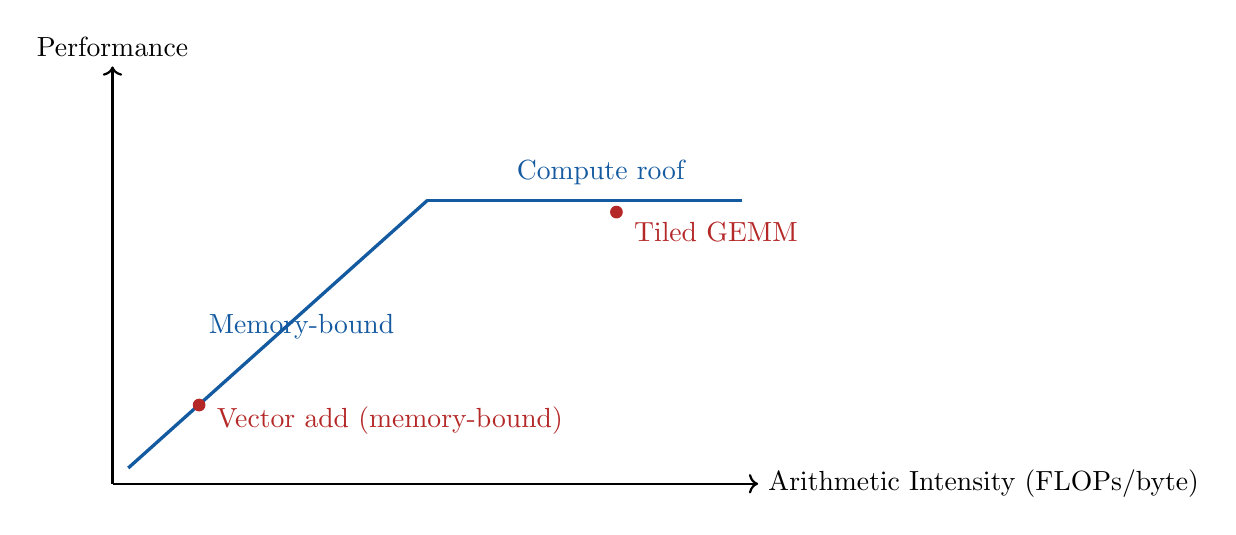
\begin{tikzpicture}[scale=1.0]
  % axes
  \draw[->, thick] (0,0) -- (8.2,0) node[right] {Arithmetic Intensity (FLOPs/byte)};
  \draw[->, thick] (0,0) -- (0,5.3) node[above] {Performance};

  % roofline
  \draw[myblue, very thick] (0.2,0.2) -- (4.0,3.6);
  \draw[myblue, very thick] (4.0,3.6) -- (8.0,3.6);

  % labels
  \node[myblue] at (2.4,2.0) {Memory-bound};
  \node[myblue] at (6.2,3.95) {Compute roof};

  % points
  \fill[myred] (1.1,1.0) circle (2.3pt);
  \node[myred, anchor=west] at (1.2,0.8) {Vector add (memory-bound)};

  \fill[myred] (6.4,3.45) circle (2.3pt);
  \node[myred, anchor=west] at (6.5,3.2) {Tiled GEMM};
\end{tikzpicture}
\end{center}

\begin{bluebox}
\textbf{Misconception cleared:} More compute does \red{not} help if you are on the memory-bound slope. First reduce bytes moved or improve locality.
\end{bluebox}

\section{Precision and Quantization}

\subsection{Why lower precision matters}

\begin{itemize}[leftmargin=1.2em]
\item Lower precision reduces model memory footprint.
\item Smaller data types increase effective memory throughput.
\item Tensor Cores typically use mixed-precision paths for speed + stability.
\end{itemize}

\subsection{FP16 vs BF16}
\begin{redbox}
\textbf{FP32 fallback and low-precision caveats (preserved):}
Some operations are sensitive and often need higher precision for numerical stability:
\begin{itemize}[leftmargin=1.2em]
\item softmax
\item normalization layers
\item attention score calculations
\item reductions
\end{itemize}
INT4 (two weights per byte) also introduces layout constraints:
\begin{itemize}[leftmargin=1.2em]
\item pack/unpack overhead
\item alignment constraints
\item avoid branch-heavy unpack logic that causes warp divergence
\end{itemize}
\end{redbox}
\begin{center}
\renewcommand{\arraystretch}{1.15}
\begin{tabular}{|p{0.22\linewidth}|p{0.33\linewidth}|p{0.37\linewidth}|}
\hline
\textbf{Format} & \textbf{Strength} & \textbf{Risk/Tradeoff} \\
\hline
FP16 & Smaller storage and high throughput & Narrow exponent range can underflow/overflow gradients \\
\hline
BF16 & FP32-like exponent range with lower precision mantissa & Less precision than FP32, but usually better training stability than FP16 \\
\hline
\end{tabular}
\end{center}

\subsection{INT8/FP8 quantization}

\begin{itemize}[leftmargin=1.2em]
\item \vocab{PTQ}: post-training quantization using calibration data.
\item \vocab{QAT}: quantization-aware training to recover accuracy.
\end{itemize}

\begin{redbox}
\textbf{Why quantization can fail or slow down (preserved + clarified):}
\begin{itemize}[leftmargin=1.2em]
\item Kernel coverage gaps force dequantize/requantize overhead.
\item If workload is compute-bound, memory savings may not move latency.
\item Accuracy can drop due to outliers and poor calibration.
\end{itemize}
\end{redbox}

Best-case path: long contiguous subgraphs remain quantized end-to-end (compiler/runtime chooses this), minimizing format conversions.

\section{Distributed Inference and Scaling Limits}

\begin{importantbox}
\textbf{Very important insert (implemented): Data Parallelism}
\begin{itemize}[leftmargin=1.2em]
\item Replicate the full model on each GPU; split inputs across replicas.
\item Common for training and also useful for high-throughput inference serving.
\item In training, gradients must be synchronized (typically with AllReduce-equivalent collectives).
\item Communication cost depends strongly on interconnect:
  NVLink/NVSwitch, PCIe, Ethernet, or InfiniBand.
\end{itemize}
\end{importantbox}

\subsection{Model parallelism}

\textbf{Pipeline parallelism:}
\begin{itemize}[leftmargin=1.2em]
\item Split layers across GPUs.
\item Can suffer from pipeline bubbles if stages are imbalanced.
\item Mitigated with micro-batching and careful schedule design.
\end{itemize}

\textbf{Tensor parallelism:}
\begin{itemize}[leftmargin=1.2em]
\item Split tensor dimensions of large matmuls across GPUs.
\item Requires frequent communication of partial results.
\item Needs high-bandwidth, low-latency links for efficiency.
\end{itemize}

\begin{center}
    \small
    \renewcommand{\arraystretch}{1.2}
    \resizebox{\linewidth}{!}{%
    \begin{tabular}{|p{0.16\linewidth}|p{0.30\linewidth}|p{0.20\linewidth}|p{0.22\linewidth}|}
    \hline
    \textbf{Collective} & \textbf{What it does} & \textbf{Common use} & \textbf{Easy recall / intuition} \\
    \hline
    Broadcast 
    & One rank sends the same data to all other ranks 
    & Weights, configs, initialization 
    & ``One → everyone'' (copy data out) \\
    \hline
    
    AllReduce 
    & Reduce across all ranks and store result in every rank 
    & Gradient synchronization (data parallel training) 
    & ``Average grads everywhere'' — each GPU trains mini-batch then syncs before update \\
    \hline
    
    Reduce 
    & Reduce across ranks, result stored in one rank only 
    & Aggregation, logging, metrics 
    & ``Everyone sends → one keeps'' \\
    \hline
    
    AllGather 
    & Gather shards so every rank ends with full data 
    & Unsharding parameters/activations (FSDP, ZeRO-3) 
    & ``Pieces → full copy on every GPU''; often after sharded training step \\
    \hline
    
    ReduceScatter 
    & Reduce first, then scatter shards so each rank keeps only a portion 
    & Sharded gradient updates (FSDP, ZeRO) 
    & ``Reduce then split'' — memory efficient; often followed by AllGather later \\
    \hline
    \end{tabular}
    }
    \end{center}
    
\subsection{Strong scaling limit}

\begin{bluebox}
\textbf{Interview framing (preserved):} At some point, adding GPUs makes each shard too small and communication dominates. Past that strong-scaling point, more GPUs can slow the job.
\end{bluebox}
\subsubsection*{\blue{Interconnect cheat sheet}}
    \begin{center}
    \renewcommand{\arraystretch}{1.15}
    \begin{tabular}{|p{0.18\linewidth}|p{0.30\linewidth}|p{0.44\linewidth}|}
    \hline
    \textbf{Tech} & \textbf{Connects} & \textbf{Why it matters} \\
    \hline
    PCIe & CPU/host $\leftrightarrow$ GPU & host-device bandwidth/latency bottleneck \\
    \hline
    NVLink & GPU $\leftrightarrow$ GPU & high bandwidth for multi-GPU on-node \\
    \hline
    InfiniBand/RDMA & node $\leftrightarrow$ node & faster distributed training communication \\
    \hline
    GPUDirect RDMA & GPU $\leftrightarrow$ NIC & avoids host copies (lower latency, less CPU overhead) \\
    \hline
    \end{tabular}
    \end{center}

\section{KV Cache and Decode Bottlenecks}

\subsubsection*{\blue{Transformer attention (Q, K, V) in plain words}}
    When the model reads each token, it creates \blue{Query (Q)}, \blue{Key (K)}, and \blue{Value (V)} vectors.
    Keys and values help the model \blue{store what this token means}. During attention, the current token's \blue{query} is compared against other tokens' \blue{keys} to decide what context matters. The model then uses the matched \blue{values} to pass forward the information that matters. This is how the model tracks context and relationships across a sentence or conversation.
    
    % ---------------------------
    % FlashAttention: tile-wise outline
    % ---------------------------
\subsubsection*{\blue{FlashAttention (tile-wise outline)}}
    Process keys/values in tiles, maintain running softmax statistics, and accumulate the output in \blue{SRAM}.


    \begin{center}
        \resizebox{\linewidth}{!}{%
        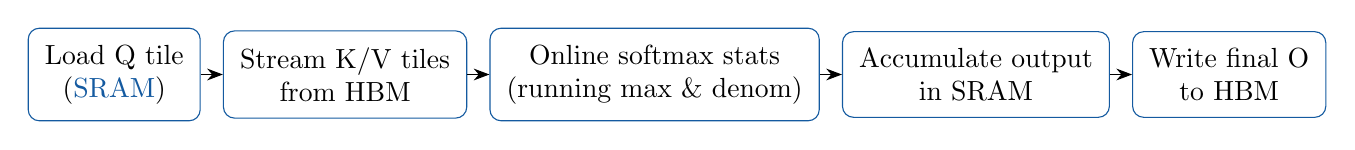
\begin{tikzpicture}[node distance=6pt]
        \node[draw=myblue, rounded corners, inner sep=6pt, align=center] (q) {Load Q tile\\(\blue{SRAM})};
        \node[draw=myblue, rounded corners, inner sep=6pt, align=center, right=8pt of q] (kv) {Stream K/V tiles\\from HBM};
        \node[draw=myblue, rounded corners, inner sep=6pt, align=center, right=8pt of kv] (soft) {Online softmax stats\\(running max \& denom)};
        \node[draw=myblue, rounded corners, inner sep=6pt, align=center, right=8pt of soft] (acc) {Accumulate output\\in SRAM};
        \node[draw=myblue, rounded corners, inner sep=6pt, align=center, right=8pt of acc] (write) {Write final O\\to HBM};
        
        \draw[-{Stealth[length=2mm]}] (q) -- (kv);
        \draw[-{Stealth[length=2mm]}] (kv) -- (soft);
        \draw[-{Stealth[length=2mm]}] (soft) -- (acc);
        \draw[-{Stealth[length=2mm]}] (acc) -- (write);
        \end{tikzpicture}
        }
        \end{center}
        
        \begin{bluebox}
        \textbf{Why it works:} keep tiles in fast memory (\blue{SRAM}), do more compute per byte loaded, and avoid materializing the full attention matrix in HBM.
        \end{bluebox}
    
        
\begin{itemize}[leftmargin=1.2em]
\item During autoregressive decoding, new tokens attend to prior context.
\item \vocab{KV cache} stores past key/value states to avoid recomputation.
\item As context grows (e.g., 10k+ tokens), KV memory traffic becomes huge.
\end{itemize}

\begin{redbox}
\textbf{Critical point:} Decode is often memory-bound because each token requires reading large KV history for relatively limited compute.
\end{redbox}

Paged attention and cache-management strategies exist to improve locality and memory efficiency.
\subsection{Prefill vs Decode}
\begin{center}
\begin{tabular}{|p{0.2\linewidth}|p{0.28\linewidth}|p{0.44\linewidth}|}
\hline
\textbf{Phase} & \textbf{Primary bottleneck} & \textbf{Best optimization levers} \\
\hline
Prefill & GEMM compute + activation memory & Better batching, tensor core utilization, graph capture, fusion \\
\hline
Decode & KV-cache bandwidth/latency & Paged KV cache, attention kernel fusion, reduced precision cache, continuous batching \\
\hline
\end{tabular}
\end{center}
\section{Compiler Stack and Kernel Fusion}

\begin{itemize}[leftmargin=1.2em]
\item Eager Python can launch many small kernels with overhead.
\item \texttt{torch.compile} and graph capture reduce interpreter overhead.
\item \vocab{Kernel fusion} combines ops (e.g., matmul + bias + activation) to reduce memory round-trips.
\end{itemize}

\begin{bluebox}
\textbf{High-impact optimization (preserved):} Fusion often shifts workloads right on the roofline plot by increasing arithmetic intensity and reducing memory traffic.
\end{bluebox}

\section{Sparsity Reality Check}

\subsection{Sparsity and Pruning}
\begin{center}
\begin{tabular}{|p{0.22\linewidth}|p{0.35\linewidth}|p{0.35\linewidth}|}
\hline
\textbf{Type} & \textbf{Description} & \textbf{Practical impact} \\
\hline
Unstructured sparsity & Removes individual weights & Often limited speedup unless specialized sparse kernels exist \\
\hline
Structured sparsity & Removes heads/channels/blocks & Better hardware mapping and real latency wins \\
\hline
\end{tabular}
\end{center}
\begin{itemize}[leftmargin=1.2em]
\item Unstructured sparsity can hurt GPU efficiency due to irregular memory access.
\item GPUs prefer regular, coalesced access patterns.
\item Structured patterns (for example, hardware-supported sparsity formats) are much easier to accelerate.
\end{itemize}
\begin{tcolorbox}[colback=insight]
    \textbf{Interview signal:} ``Sparsity is only useful when compiler + kernel + hardware path is sparse-aware.''
    \end{tcolorbox}
    
\section{Numerical Stability and Reproducibility}

\begin{itemize}[leftmargin=1.2em]
\item Floating-point addition is not associative in practice.
\item Different reduction orders across devices can produce different results.
\item Distributed collectives may be non-deterministic unless explicitly constrained.
\end{itemize}

Subnormal handling note (preserved + clarified): denormal/subnormal numbers can be very slow on some hardware paths. Flush-to-zero behavior can improve speed but may change tiny-value numerics; treat as a controlled tradeoff.

\section{Final Mental Model}

\begin{redbox}
Performance engineering is constant tradeoff management:
\begin{itemize}[leftmargin=1.2em]
\item compute vs memory traffic

\begin{center}
    \renewcommand{\arraystretch}{1.15}
    \resizebox{\linewidth}{!}{%
    \begin{tabular}{|p{0.20\linewidth}|p{0.36\linewidth}|p{0.36\linewidth}|}
    \hline
    \textbf{Regime} & \textbf{What you see} & \textbf{What you do} \\
    \hline
    Compute-bound & high SM active, BW not maxed, kernels dominate runtime & increase tensor core use, fuse kernels, improve occupancy, reduce divergence \\
    \hline
    Memory-bound & BW near peak, moderate SM active, lots of stalls & tiling, shared memory/cache reuse, coalescing, fewer global reads/writes, cachce misses\\
    \hline
    I/O-bound & GPU idle, data loader maxed, disk/network busy & dataset caching, preprocessing offline, parallel data loaders; faster storage (SSD/NVMe), reduced contention, and distributed data sharding with node-local caching \\
    \hline
    \end{tabular}
    }
    \end{center}
\item communication vs parallelism
\item numerical fidelity vs throughput
\item Python-level abstraction vs hardware-level control
\end{itemize}
As Moore's law slows, gains increasingly come from software-hardware co-design and careful systems optimization.
\end{redbox}
\subsection*{\blue{Profiling Section}}
\subsection{Profiling / Debugging Cheat Sheet}

\begin{center}
\renewcommand{\arraystretch}{1.2}
\begin{tabular}{|p{0.26\linewidth}|p{0.64\linewidth}|}
\hline
\textbf{Tool / Snippet} & \textbf{Meaning (clean + interview-ready)} \\
\hline
\blue{\textbf{Nsight Systems (nsys)}} & End-to-end timeline: CPU$\leftrightarrow$GPU overlap, kernel launches, synchronization, memcpy, data loader stalls. \\
\hline
\blue{\textbf{Nsight Compute (ncu)}} & Deep kernel analysis: occupancy, memory throughput, instruction mix, warp stalls, cache behavior. \\
\hline
\blue{\textbf{cuda-gdb}} & Debug CUDA kernels (breakpoints, stepping, inspecting variables). \\
\hline
\blue{\textbf{cuda-memcheck}} & Memory correctness: out-of-bounds, invalid accesses, (some) race-like issues. \\
\hline
\blue{\textbf{CUDA runtime + driver APIs}} &
Managing devices, memory, and program execution on the GPU. \\
\hline
\blue{\textbf{cudaMalloc(\dots)}} & Allocates memory on the \textbf{GPU}. (\texttt{malloc} allocates on \textbf{CPU}.) \\
\hline
\blue{\textbf{cudaMemcpy(\dots)}} & Copies data \textbf{CPU$\leftrightarrow$GPU} (host-device transfers). \\
\hline
\end{tabular}
\end{center}

\begin{redbox}
\textbf{Fast rule:} \blue{nsys} tells you \emph{where time goes overall}. \blue{ncu} tells you \emph{why a specific kernel is slow}.
\end{redbox}

\subsection{Nsight Compute (NCU) Quick Commands}

\begin{bluebox}
\textbf{Use NCU to answer:} am I \blue{compute-bound} or \blue{memory-bound}, and what limits occupancy/stalls?
\end{bluebox}

\begin{center}
\renewcommand{\arraystretch}{1.2}
\begin{tabular}{|p{0.38\linewidth}|p{0.52\linewidth}|}
\hline
\textbf{What you want} & \textbf{Command} \\
\hline
Profile app (basic) & \texttt{ncu ./vecAdd} \\
\hline
Fuller kernel metrics (heavier) & \texttt{ncu --set full ./vecAdd} \\
\hline
Profile only one kernel by name & \texttt{ncu -k vecAdd ./vecAdd} \\
\hline
Save report file & \texttt{ncu -o report\_vecAdd ./vecAdd} \\
\hline
Reduce overhead (often faster) & \texttt{ncu --replay-mode application ./vecAdd} \\
\hline
\end{tabular}
\end{center}

%%%%%%%%%%%%%%%%%%%%%%%%%%%%%%%%%%%%%%%%%%%%%%%%%%%%%%%%%%%%
% 4) CUDA INDEXING QUICK RECALL (cleaned)
%%%%%%%%%%%%%%%%%%%%%%%%%%%%%%%%%%%%%%%%%%%%%%%%%%%%%%%%%%%%
\subsection{CUDA Indexing (Fast Recall)}

\begin{center}
\renewcommand{\arraystretch}{1.2}
\begin{tabular}{|p{0.30\linewidth}|p{0.60\linewidth}|}
\hline
\textbf{Name} & \textbf{Meaning} \\
\hline
\texttt{gridDim.x}, \texttt{gridDim.y} & How many blocks wide/tall in the launched grid. \\
\hline
\texttt{blockDim.x}, \texttt{blockDim.y} & Threads per block in x/y. \\
\hline
\texttt{threadIdx.x}, \texttt{threadIdx.y} & Thread’s local coordinates inside its block. \\
\hline
\texttt{blockIdx.x}, \texttt{blockIdx.y} & Block’s coordinates inside the grid. \\
\hline
\end{tabular}
\end{center}

\begin{bluebox}
\textbf{2D output indexing (matmul / conv-style):}\\
\[
\begin{aligned}
i &= \texttt{blockIdx.y}\cdot\texttt{blockDim.y} + \texttt{threadIdx.y} \\
j &= \texttt{blockIdx.x}\cdot\texttt{blockDim.x} + \texttt{threadIdx.x}
\end{aligned}
\]
\end{bluebox}
\subsection{Cluster Launch (Slurm) — \texttt{srun} Line Breakdown}

\begin{bluebox}
\textbf{Command (preserved):}\\
\texttt{srun --partition=gpu --gres=gpu:1 --mem=16G --time=01:00:00 --pty bash}
\end{bluebox}

\begin{center}
\renewcommand{\arraystretch}{1.2}
\begin{tabular}{|p{0.30\linewidth}|p{0.60\linewidth}|}
\hline
\textbf{Flag} & \textbf{What it does} \\
\hline
\texttt{--partition=gpu} & Run on the GPU partition/queue. \\
\hline
\texttt{--gres=gpu:1} & Request 1 GPU resource. \\
\hline
\texttt{--mem=16G} & Request 16 GB of system RAM. \\
\hline
\texttt{--time=01:00:00} & Time limit of 1 hour. \\
\hline
\texttt{--pty bash} & Start an interactive pseudo-terminal (a shell) on the allocated node. \\
\hline
\end{tabular}
\end{center}

\begin{redbox}
\textbf{Interview phrasing:} “\texttt{srun --pty} is how I grab an interactive GPU node to debug quickly before running a long \texttt{sbatch} job.”
\end{redbox}

insert CCUDA AMTMUL SECTION:
\subsection{Naive Matrix Multiply (CPU + CUDA) — Interview Baseline}

\begin{bluebox}
\textbf{Purpose:} show you understand indexing, memory layout, and where the bottleneck comes from.  
This is \red{naive} (no tiling/shared memory). Optimizations come after.
\end{bluebox}

\subsubsection*{\blue{CPU Naive Matmul (row-major)}}
\begin{verbatim}
void matmul_cpu(const float* A, const float* B, float* C,
                int M, int K, int N) {
  // A: MxK, B: KxN, C: MxN (row-major)
  for (int i = 0; i < M; i++) {
    for (int j = 0; j < N; j++) {
      float sum = 0.0f;
      for (int k = 0; k < K; k++) {
        sum += A[i*K + k] * B[k*N + j];
      }
      C[i*N + j] = sum;
    }
  }
}
\end{verbatim}

\subsubsection*{\blue{CUDA Naive Matmul Kernel}}
\begin{verbatim}
__global__ void matmul_cuda(const float* A, const float* B, float* C,
                            int M, int K, int N) {
  int i = blockIdx.y * blockDim.y + threadIdx.y; // row
  int j = blockIdx.x * blockDim.x + threadIdx.x; // col

  if (i < M && j < N) {
    float sum = 0.0f;
    for (int k = 0; k < K; k++) {
      sum += A[i*K + k] * B[k*N + j];
    }
    C[i*N + j] = sum;
  }
}
\end{verbatim}

\subsubsection*{\blue{Launch Configuration (simple)}}
\begin{verbatim}
// Example: 16x16 threads per block
dim3 block(16, 16);
dim3 grid((N + block.x - 1) / block.x,
          (M + block.y - 1) / block.y);

matmul_cuda<<<grid, block>>>(A, B, C, M, K, N);
\end{verbatim}

\begin{redbox}
\textbf{What makes this naive kernel slow:}
\begin{itemize}
\item Each thread re-loads A/B from global memory many times (low data reuse).
\item No shared-memory tiling, so memory traffic is high.
\item Typically becomes \blue{memory-bound} at scale (unless extremely small sizes).
\end{itemize}
\end{redbox}

%%%%%%%%%%%%%%%%%%%%%%%%%%%%%%%%%%%%%%%%%%%%%%%%%%%%%%%%%%%%
\subsection{Simple Tiling + Shared Memory Optimization (next step)}
%%%%%%%%%%%%%%%%%%%%%%%%%%%%%%%%%%%%%%%%%%%%%%%%%%%%%%%%%%%%

\begin{bluebox}
\textbf{Goal:} reuse global memory loads by staging tiles of $A$ and $B$ in \blue{shared memory}.\\
Each block loads a small tile once, then reuses it for many MACs.
\end{bluebox}

\subsubsection*{\blue{Tiled CUDA Matmul (shared memory)}}
\begin{verbatim}
#define TILE 16

__global__ void matmul_tiled(const float* A, const float* B, float* C,
                             int M, int K, int N) {
  __shared__ float As[TILE][TILE];
  __shared__ float Bs[TILE][TILE];

  int row = blockIdx.y * TILE + threadIdx.y;
  int col = blockIdx.x * TILE + threadIdx.x;

  float sum = 0.0f;

  // Loop over tiles in the K dimension
  for (int t = 0; t < (K + TILE - 1) / TILE; t++) {

    int a_col = t * TILE + threadIdx.x; // k index for A
    int b_row = t * TILE + threadIdx.y; // k index for B

    // Load A and B tiles into shared memory (with bounds checks)
    As[threadIdx.y][threadIdx.x] =
        (row < M && a_col < K) ? A[row * K + a_col] : 0.0f;

    Bs[threadIdx.y][threadIdx.x] =
        (b_row < K && col < N) ? B[b_row * N + col] : 0.0f;

    __syncthreads(); // ensure tiles are loaded before compute

    // Compute partial dot product for this tile
    #pragma unroll
    for (int k = 0; k < TILE; k++) {
      sum += As[threadIdx.y][k] * Bs[k][threadIdx.x];
    }

    __syncthreads(); // ensure all threads finished before loading next tile
  }

  if (row < M && col < N) {
    C[row * N + col] = sum;
  }
}
\end{verbatim}

\subsubsection*{\blue{Launch Configuration (tiled)}}
\begin{verbatim}
dim3 block(TILE, TILE);
dim3 grid((N + TILE - 1) / TILE,
          (M + TILE - 1) / TILE);

matmul_tiled<<<grid, block>>>(A, B, C, M, K, N);
\end{verbatim}

\begin{redbox}
\textbf{Why shared-memory tiling is faster (simple recall):}
\begin{itemize}
\item \blue{Global → shared once per tile}, then reused many times.
\item Much higher \blue{arithmetic intensity} (more FLOPs per byte loaded).
\item Less pressure on HBM/global bandwidth → closer to compute-bound.
\end{itemize}
\end{redbox}

\section*{\blue{Experience Section}}
%%%%%%%%%%%%%%%%%%%%%%%%%%%%%%%%%%%%%%%%%%%%%%%%%%%%%%%%%%%%
\ProjectHeader{HPC Workflows: Multi-GPU Training + Benchmarking (WAVE HPC Support Experience)}{Slurm, Kubernetes, GPU clusters, distributed ML infrastructure}
%%%%%%%%%%%%%%%%%%%%%%%%%%%%%%%%%%%%%%%%%%%%%%%%%%%%%%%%%%%%

\subsection{Short Pitch}
I worked on designing and supporting HPC workflows for multi-GPU training, benchmarking, and cluster resource optimization while also serving as a support engineer on the WAVE HPC cluster. The role involved helping users run distributed ML workloads, troubleshooting job scheduling issues, and improving GPU utilization through better profiling, scheduling practices, and workflow design.

\subsection{Why I Did It + What I Learned}
I wanted hands-on exposure to real GPU cluster infrastructure beyond just running experiments myself, and working in a support role at WAVE gave me visibility into how many different workloads behave at scale. It helped me understand how scheduling policies, communication overhead, data pipelines, and storage systems affect distributed deep learning performance. Supporting other users also strengthened my ability to explain HPC concepts in a beginner-friendly way while still thinking from a systems and performance perspective.

\subsection{Challenges}
One challenge was diagnosing distributed training slowdowns, which often came from communication overhead, data loading bottlenecks, or misconfigured jobs rather than compute limits. Load balancing across GPUs and nodes also required careful monitoring. Another challenge was ensuring reproducibility across environments, since differences in drivers, libraries, and cluster configurations could affect results.

\subsection{Key Interview Takeaways}
A key idea I emphasize is that scaling ML workloads introduces communication and infrastructure bottlenecks that can offset raw compute gains. Efficient cluster usage often requires profiling, scheduling optimization, and good workflow design, not just bigger models or faster GPUs. My WAVE support experience reinforced how real-world HPC systems operate and how to think about performance from both the user and infrastructure perspective.

\ProjectHeader{Research: LLMCompass — Computational Graph Exploration Across LLMs and Hardware}{LLM systems, hardware–model co-design, inference optimization, GPU/HPC performance}
%%%%%%%%%%%%%%%%%%%%%%%%%%%%%%%%%%%%%%%%%%%%%%%%%%%%%%%%%%%%

\subsection{Short Pitch (GPU / HPC Focus)}
I worked on LLMCompass, a research-oriented computational graph tool designed to explore how different large language models map onto different hardware systems. The goal was to build intuition around how model architecture, inference strategies, and hardware characteristics interact, especially in terms of GPU utilization, memory bandwidth, and system throughput.

\subsection{Why I Did It + What I Learned}
I wanted a beginner-friendly but research-grounded way to understand how LLM inference actually behaves on real hardware beyond just reading papers. Working on LLMCompass helped me see how computational graphs translate into memory movement, compute patterns, and scaling behavior. I gained intuition about how model structure, batching, and hardware characteristics influence overall performance.

\subsection{Challenges}
One challenge was understanding how different hardware constraints change the optimal computational graph design. Another was learning to interpret performance tradeoffs without assuming one model or hardware setup is universally best. I also worked on keeping explanations accessible so newer students could use the tool to build systems intuition.

\subsection{Key Interview Takeaways}
A key idea I emphasize is that LLM performance is heavily shaped by the interaction between model architecture and hardware capabilities, not just model size alone. Computational graphs help visualize these tradeoffs, making it easier to reason about bottlenecks like memory bandwidth, compute utilization, and scaling across accelerators.
%%%%%%%%%%%%%%%%%%%%%%%%%%%%%%%%%%%%%%%%%%%%%%%%%%%%%%%%%%%%
\ProjectHeader{Research: Convolution Optimization with Triton}{Triton, CUDA, PyTorch, GPU kernel optimization, memory hierarchy}
%%%%%%%%%%%%%%%%%%%%%%%%%%%%%%%%%%%%%%%%%%%%%%%%%%%%%%%%%%%%

\subsection{Short Pitch}
I worked on implementing custom Triton kernels for 2D convolution layers to better understand how deep learning workloads map onto GPUs. The project focused on exploring memory hierarchy, tiling strategies, and thread mapping to improve GPU utilization and reduce kernel overhead compared to standard PyTorch convolution operations.

\subsection{Why I Did It + What I Learned}
I wanted hands-on experience writing GPU kernels in a way that was beginner-friendly but still grounded in real performance research. Since most frameworks rely on cuDNN as a black box, this helped me build intuition about how convolutions actually execute on hardware. I learned how memory access patterns, tiling, and warp-level execution influence performance, and developed a stronger understanding of GPU memory locality, tensor core usage, and kernel scheduling tradeoffs.

\subsection{Challenges}
One challenge was balancing occupancy with shared memory and register limits while still maintaining good performance. Debugging correctness while optimizing speed was also tricky, especially when working with custom kernel implementations. Another challenge was understanding when the kernel was compute-bound versus memory-bound and how that affected optimization decisions.

\subsection{Key Interview Takeaways}
A key idea I emphasize is that GPU kernel optimization is largely about memory locality and efficient data movement rather than just raw compute. Writing Triton kernels made it much clearer how tiling, coalesced memory access, and batching influence throughput, and why profiling tools like Nsight Compute are essential for understanding performance bottlenecks.

%%%%%%%%%%%%%%%%%%%%%%%%%%%%%%%%%%%%%%%%%%%%%%%%%%%%%%%%%%%%
\ProjectHeader{GPU-Accelerated Image Processing Pipeline}{CUDA, PyTorch, GPU kernels, memory optimization, V100 GPUs}
%%%%%%%%%%%%%%%%%%%%%%%%%%%%%%%%%%%%%%%%%%%%%%%%%%%%%%%%%%%%

\subsection{Short Pitch}
I built a GPU-accelerated image processing pipeline implementing blur and sharpen filters using custom CUDA kernels, achieving up to an 8× speedup over CPU baselines. The project focused on understanding how image processing workloads map onto GPUs and how memory access patterns influence performance.

\subsection{Why I Did It + What I Learned}
I wanted strong GPU fundamentals before going deeper into ML systems work, so this project was intentionally beginner-friendly but grounded in real performance engineering. It helped me understand kernel launch configuration, GPU memory hierarchy, profiling workflows, and when GPU acceleration is actually worthwhile. I also developed intuition about data locality, host-device transfers, and how preprocessing pipelines interact with GPU compute.

\subsection{Challenges}
One challenge was optimizing memory access patterns so threads could efficiently process image pixels without excessive global memory traffic. Avoiding unnecessary CPU–GPU transfers was another important factor for performance. I also focused on stable benchmarking across different image sizes while validating GPU outputs against CPU reference implementations to ensure correctness.

\subsection{Key Interview Takeaways}
A key idea I emphasize is that GPU performance is often limited more by memory movement than raw compute, especially in image processing pipelines. Writing custom CUDA kernels made it clearer how thread mapping, shared memory caching, and memory coalescing directly affect throughput and why profiling is essential when optimizing GPU workloads.
%%%%%%%%%%%%%%%%%%%%%%%%%%%%%%%%%%%%%%%%%%%%%%%%%%%%%%%%%%%%
\ProjectHeader{High-Performance Matrix Inversion via Custom GPU Kernels}{Triton, OpenCL, C++, GPU linear algebra, HPC optimization}
%%%%%%%%%%%%%%%%%%%%%%%%%%%%%%%%%%%%%%%%%%%%%%%%%%%%%%%%%%%%

\subsection{Short Pitch}
I worked on implementing GPU-based matrix inversion kernels for large matrices, focusing on how numerical linear algebra workloads map onto GPU hardware. The project explored parallel decomposition strategies, memory reuse, and kernel design to reduce runtime compared to traditional CPU-based numerical implementations while building intuition around HPC-style compute patterns relevant to machine learning systems.

\subsection{Why I Did It + What I Learned}
I wanted a beginner-friendly but research-grounded way to understand how foundational linear algebra operations — like matrix inversion and multiplication — connect directly to deep learning performance. This project helped me see how many ML workloads ultimately reduce to optimized matrix operations, and how GPU kernel design, tiling, and memory hierarchy decisions impact both training and inference efficiency. I also gained perspective on portability versus performance by experimenting with both Triton and OpenCL approaches.

\subsection{Technical Implementation (Code Logic)}
The implementation partitions matrices into blocks processed in parallel by GPU threads, where each thread block performs partial inversion or elimination steps. Shared memory is used to cache intermediate values and reduce global memory traffic, while synchronization ensures correctness across blocks. I also explored kernel fusion techniques to minimize intermediate writes, and compared OpenCL implementations to understand tradeoffs between cross-platform portability and peak GPU performance.

\subsection{Challenges}
Maintaining numerical stability while pushing for performance was one of the main challenges, especially when balancing precision and throughput. Synchronization overhead, memory reuse patterns, and choosing appropriate block sizes also required careful tuning. Comparing different frameworks introduced additional complexity around portability and optimization tradeoffs.

\subsection{Key Interview Takeaways}
A key idea I emphasize is that many large-scale ML workloads are fundamentally linear algebra problems, so optimizing these primitives directly impacts system performance. This project reinforced how kernel tiling, synchronization strategy, memory locality, and precision management all play major roles in GPU efficiency and scalability.

%%%%%%%%%%%%%%%%%%%%%%%%%%%%%%%%%%%%%%%%%%%%%%%%%%%%%%%%%%%%
\ProjectHeader{LABUBU AI Shopper}{LLMs, vector search, FastAPI, React, Faiss, RAG systems}
%%%%%%%%%%%%%%%%%%%%%%%%%%%%%%%%%%%%%%%%%%%%%%%%%%%%%%%%%%%%

\subsection{Short Pitch}
I built LABUBU AI Shopper, a real-time AI shopping assistant that combines vector search with LLM prompting to help users find products conversationally. The system handled around 1000 SKUs with sub-second response times, focusing on making LLM-powered retrieval practical for a production-style application.

\subsection{Why I Did It + What I Learned}
I wanted hands-on experience building a full LLM application stack in a way that was beginner-friendly but still reflective of real production systems. Through this project, I learned prompt engineering, retrieval-augmented generation design, and latency optimization across both the vector search and inference pipeline. It also gave me a better intuition for the tradeoffs between embedding search cost, caching strategies, and overall response speed.

\subsection{Challenges}
One challenge was managing latency across multiple stages — retrieval, reranking, and LLM inference — while keeping responses fast enough for real-time interaction. Scaling the vector search while maintaining result quality was another consideration. I also focused on designing a reliable API workflow so the frontend and backend stayed responsive under load.

\subsection{Key Interview Takeaways}
A key idea I emphasize is that in many real LLM systems, retrieval latency can dominate inference latency, so optimizing data flow and caching is just as important as optimizing the model itself. Building this system helped me understand how RAG pipelines work end-to-end and how architectural decisions affect both performance and user experience.

\end{document}
